% Options for packages loaded elsewhere
\PassOptionsToPackage{unicode}{hyperref}
\PassOptionsToPackage{hyphens}{url}
\PassOptionsToPackage{dvipsnames,svgnames,x11names}{xcolor}
%
\documentclass[
  letterpaper,
  DIV=11,
  numbers=noendperiod]{scrartcl}

\usepackage{amsmath,amssymb}
\usepackage{iftex}
\ifPDFTeX
  \usepackage[T1]{fontenc}
  \usepackage[utf8]{inputenc}
  \usepackage{textcomp} % provide euro and other symbols
\else % if luatex or xetex
  \usepackage{unicode-math}
  \defaultfontfeatures{Scale=MatchLowercase}
  \defaultfontfeatures[\rmfamily]{Ligatures=TeX,Scale=1}
\fi
\usepackage{lmodern}
\ifPDFTeX\else  
    % xetex/luatex font selection
\fi
% Use upquote if available, for straight quotes in verbatim environments
\IfFileExists{upquote.sty}{\usepackage{upquote}}{}
\IfFileExists{microtype.sty}{% use microtype if available
  \usepackage[]{microtype}
  \UseMicrotypeSet[protrusion]{basicmath} % disable protrusion for tt fonts
}{}
\makeatletter
\@ifundefined{KOMAClassName}{% if non-KOMA class
  \IfFileExists{parskip.sty}{%
    \usepackage{parskip}
  }{% else
    \setlength{\parindent}{0pt}
    \setlength{\parskip}{6pt plus 2pt minus 1pt}}
}{% if KOMA class
  \KOMAoptions{parskip=half}}
\makeatother
\usepackage{xcolor}
\setlength{\emergencystretch}{3em} % prevent overfull lines
\setcounter{secnumdepth}{5}
% Make \paragraph and \subparagraph free-standing
\makeatletter
\ifx\paragraph\undefined\else
  \let\oldparagraph\paragraph
  \renewcommand{\paragraph}{
    \@ifstar
      \xxxParagraphStar
      \xxxParagraphNoStar
  }
  \newcommand{\xxxParagraphStar}[1]{\oldparagraph*{#1}\mbox{}}
  \newcommand{\xxxParagraphNoStar}[1]{\oldparagraph{#1}\mbox{}}
\fi
\ifx\subparagraph\undefined\else
  \let\oldsubparagraph\subparagraph
  \renewcommand{\subparagraph}{
    \@ifstar
      \xxxSubParagraphStar
      \xxxSubParagraphNoStar
  }
  \newcommand{\xxxSubParagraphStar}[1]{\oldsubparagraph*{#1}\mbox{}}
  \newcommand{\xxxSubParagraphNoStar}[1]{\oldsubparagraph{#1}\mbox{}}
\fi
\makeatother


\providecommand{\tightlist}{%
  \setlength{\itemsep}{0pt}\setlength{\parskip}{0pt}}\usepackage{longtable,booktabs,array}
\usepackage{calc} % for calculating minipage widths
% Correct order of tables after \paragraph or \subparagraph
\usepackage{etoolbox}
\makeatletter
\patchcmd\longtable{\par}{\if@noskipsec\mbox{}\fi\par}{}{}
\makeatother
% Allow footnotes in longtable head/foot
\IfFileExists{footnotehyper.sty}{\usepackage{footnotehyper}}{\usepackage{footnote}}
\makesavenoteenv{longtable}
\usepackage{graphicx}
\makeatletter
\def\maxwidth{\ifdim\Gin@nat@width>\linewidth\linewidth\else\Gin@nat@width\fi}
\def\maxheight{\ifdim\Gin@nat@height>\textheight\textheight\else\Gin@nat@height\fi}
\makeatother
% Scale images if necessary, so that they will not overflow the page
% margins by default, and it is still possible to overwrite the defaults
% using explicit options in \includegraphics[width, height, ...]{}
\setkeys{Gin}{width=\maxwidth,height=\maxheight,keepaspectratio}
% Set default figure placement to htbp
\makeatletter
\def\fps@figure{htbp}
\makeatother

\KOMAoption{captions}{tableheading}
\makeatletter
\@ifpackageloaded{caption}{}{\usepackage{caption}}
\AtBeginDocument{%
\ifdefined\contentsname
  \renewcommand*\contentsname{Table of contents}
\else
  \newcommand\contentsname{Table of contents}
\fi
\ifdefined\listfigurename
  \renewcommand*\listfigurename{List of Figures}
\else
  \newcommand\listfigurename{List of Figures}
\fi
\ifdefined\listtablename
  \renewcommand*\listtablename{List of Tables}
\else
  \newcommand\listtablename{List of Tables}
\fi
\ifdefined\figurename
  \renewcommand*\figurename{Figure}
\else
  \newcommand\figurename{Figure}
\fi
\ifdefined\tablename
  \renewcommand*\tablename{Table}
\else
  \newcommand\tablename{Table}
\fi
}
\@ifpackageloaded{float}{}{\usepackage{float}}
\floatstyle{ruled}
\@ifundefined{c@chapter}{\newfloat{codelisting}{h}{lop}}{\newfloat{codelisting}{h}{lop}[chapter]}
\floatname{codelisting}{Listing}
\newcommand*\listoflistings{\listof{codelisting}{List of Listings}}
\makeatother
\makeatletter
\makeatother
\makeatletter
\@ifpackageloaded{caption}{}{\usepackage{caption}}
\@ifpackageloaded{subcaption}{}{\usepackage{subcaption}}
\makeatother

\ifLuaTeX
  \usepackage{selnolig}  % disable illegal ligatures
\fi
\usepackage{bookmark}

\IfFileExists{xurl.sty}{\usepackage{xurl}}{} % add URL line breaks if available
\urlstyle{same} % disable monospaced font for URLs
\hypersetup{
  pdftitle={Supplement to Example Manuscript Template for a Data Analysis Project},
  colorlinks=true,
  linkcolor={blue},
  filecolor={Maroon},
  citecolor={Blue},
  urlcolor={Blue},
  pdfcreator={LaTeX via pandoc}}


\title{Supplement to Example Manuscript Template for a Data Analysis
Project}
\author{}
\date{}

\begin{document}
\maketitle


\section{Overview}\label{overview}

This supplementary material provides additional details, analyses, and
outputs supporting the findings presented in the main manuscript. It
includes extended methodological explanations, reproducibility
instructions, and results from exploratory data analysis. Key
supplementary tables and figures include variable summaries, survival
modeling outputs, and machine learning performance metrics. Detailed
results from Cox regression, Random Forest, and LASSO Cox models are
presented along with confusion matrices, AUC values, and variable
importance rankings. The structure and content of the project directory
are outlined to facilitate full reproducibility. Together, these
materials offer a comprehensive view of the analytical workflow and
support the robustness of the study's conclusions.

\section{Code and file information}\label{code-and-file-information}

This project is organized in a modular and reproducible structure,
separating raw data, processing scripts, analysis outputs, and final
products. Below is a guide to the directory structure and instructions
to reproduce all results.

\subsubsection{Directory Structure
Overview}\label{directory-structure-overview}

ZUBER-MADA-project/ │ ├── data/ │ ├── raw-data/ \# Contains the original
input datasets (raw files) │ └── processed-data/ \# Contains the cleaned
and transformed datasets │ ├── code/ │ ├── processing-code/ \# Data
cleaning scripts │ ├── eda-code/ \# Exploratory data analysis scripts │
└── analysis-code/ \# Statistical modeling and prediction │ ├── results/
│ ├── edatables/ \# Exploratory summary tables │ ├── edafigures/ \#
Exploratory plots │ ├── tables/ \# Model results tables │ ├── figures/
\# Model-related figures │ └── output/ \# Rendered final outputs
(PDF/HTML) │ ├── products/ │ ├── manuscript/ \# Manuscript and
supplementary files │ ├── poster/ \# Poster material (if applicable) │
└── slides/ \# Presentation slides (if applicable) │ ├── assets/ \#
Bibliography and citation style files └── README.md \# Project overview
and general usage instructions

\newpage{}

\section{Additional Method Details}\label{additional-method-details}

Often, the main manuscript only allows for an overview description of
the methods. Use the supplement to describe all your methods, models and
approaches in a lot of detail. Reference specific parts of your code as
needed.

\newpage{}

\section{Additional results}\label{additional-results}

Show additional results here. Those can be some useful
exploratory/descriptive figures or tables, or results from additional
analyses that didn't make it into the main text.

\section{Additional result}\label{additional-result}

\subsection{Exploratory Analysis:Race
Distribution}\label{exploratory-analysisrace-distribution}

As part of the descriptive exploration of the dataset, we examined the
distribution of patients by race. The majority of patients in the cohort
identified as White, followed by Black, Asian or Pacific Islander,
American Indian/Alaska Native, and a small proportion with unknown race
information. Table~\ref{tbl-race-summary}. Frequency distribution of
patients across racial categories.

\begin{longtable}[]{@{}lr@{}}

\caption{\label{tbl-race-summary}Distribution of patients by race in the
analytic cohort.}

\tabularnewline

\toprule\noalign{}
race & Count \\
\midrule\noalign{}
\endhead
\bottomrule\noalign{}
\endlastfoot
American Indian/Alaska Native & 38 \\
Asian or Pacific Islander & 506 \\
Black & 1028 \\
Unknown & 12 \\
White & 4124 \\

\end{longtable}

\subsection{Exploratory Summary: Year of
Diagnosis}\label{exploratory-summary-year-of-diagnosis}

We also summarized the distribution of patients by year of cancer
diagnosis to understand the temporal spread of the study cohort. This
information helps contextualize potential changes in treatment patterns,
diagnostic advancements, or survival outcomes over time.
Table~\ref{tbl-year-summary}. Frequency distribution of patients by year
of diagnosis.

\begin{longtable}[]{@{}lr@{}}

\caption{\label{tbl-year-summary}Distribution of patients by year of
diagnosis.}

\tabularnewline

\toprule\noalign{}
diagnosis\_year & Count \\
\midrule\noalign{}
\endhead
\bottomrule\noalign{}
\endlastfoot
2010 & 821 \\
2011 & 889 \\
2012 & 960 \\
2013 & 972 \\
2014 & 962 \\
2015 & 1104 \\

\end{longtable}

\begin{enumerate}
\def\labelenumi{\arabic{enumi}.}
\tightlist
\item
  Bar plot displaying the distribution of patients by year of diagnosis.
  The figure shows a relatively even spread across the years, with some
  fluctuations that may reflect data entry trends or cohort recruitment
  variability.
\end{enumerate}

\begin{figure}

\centering{

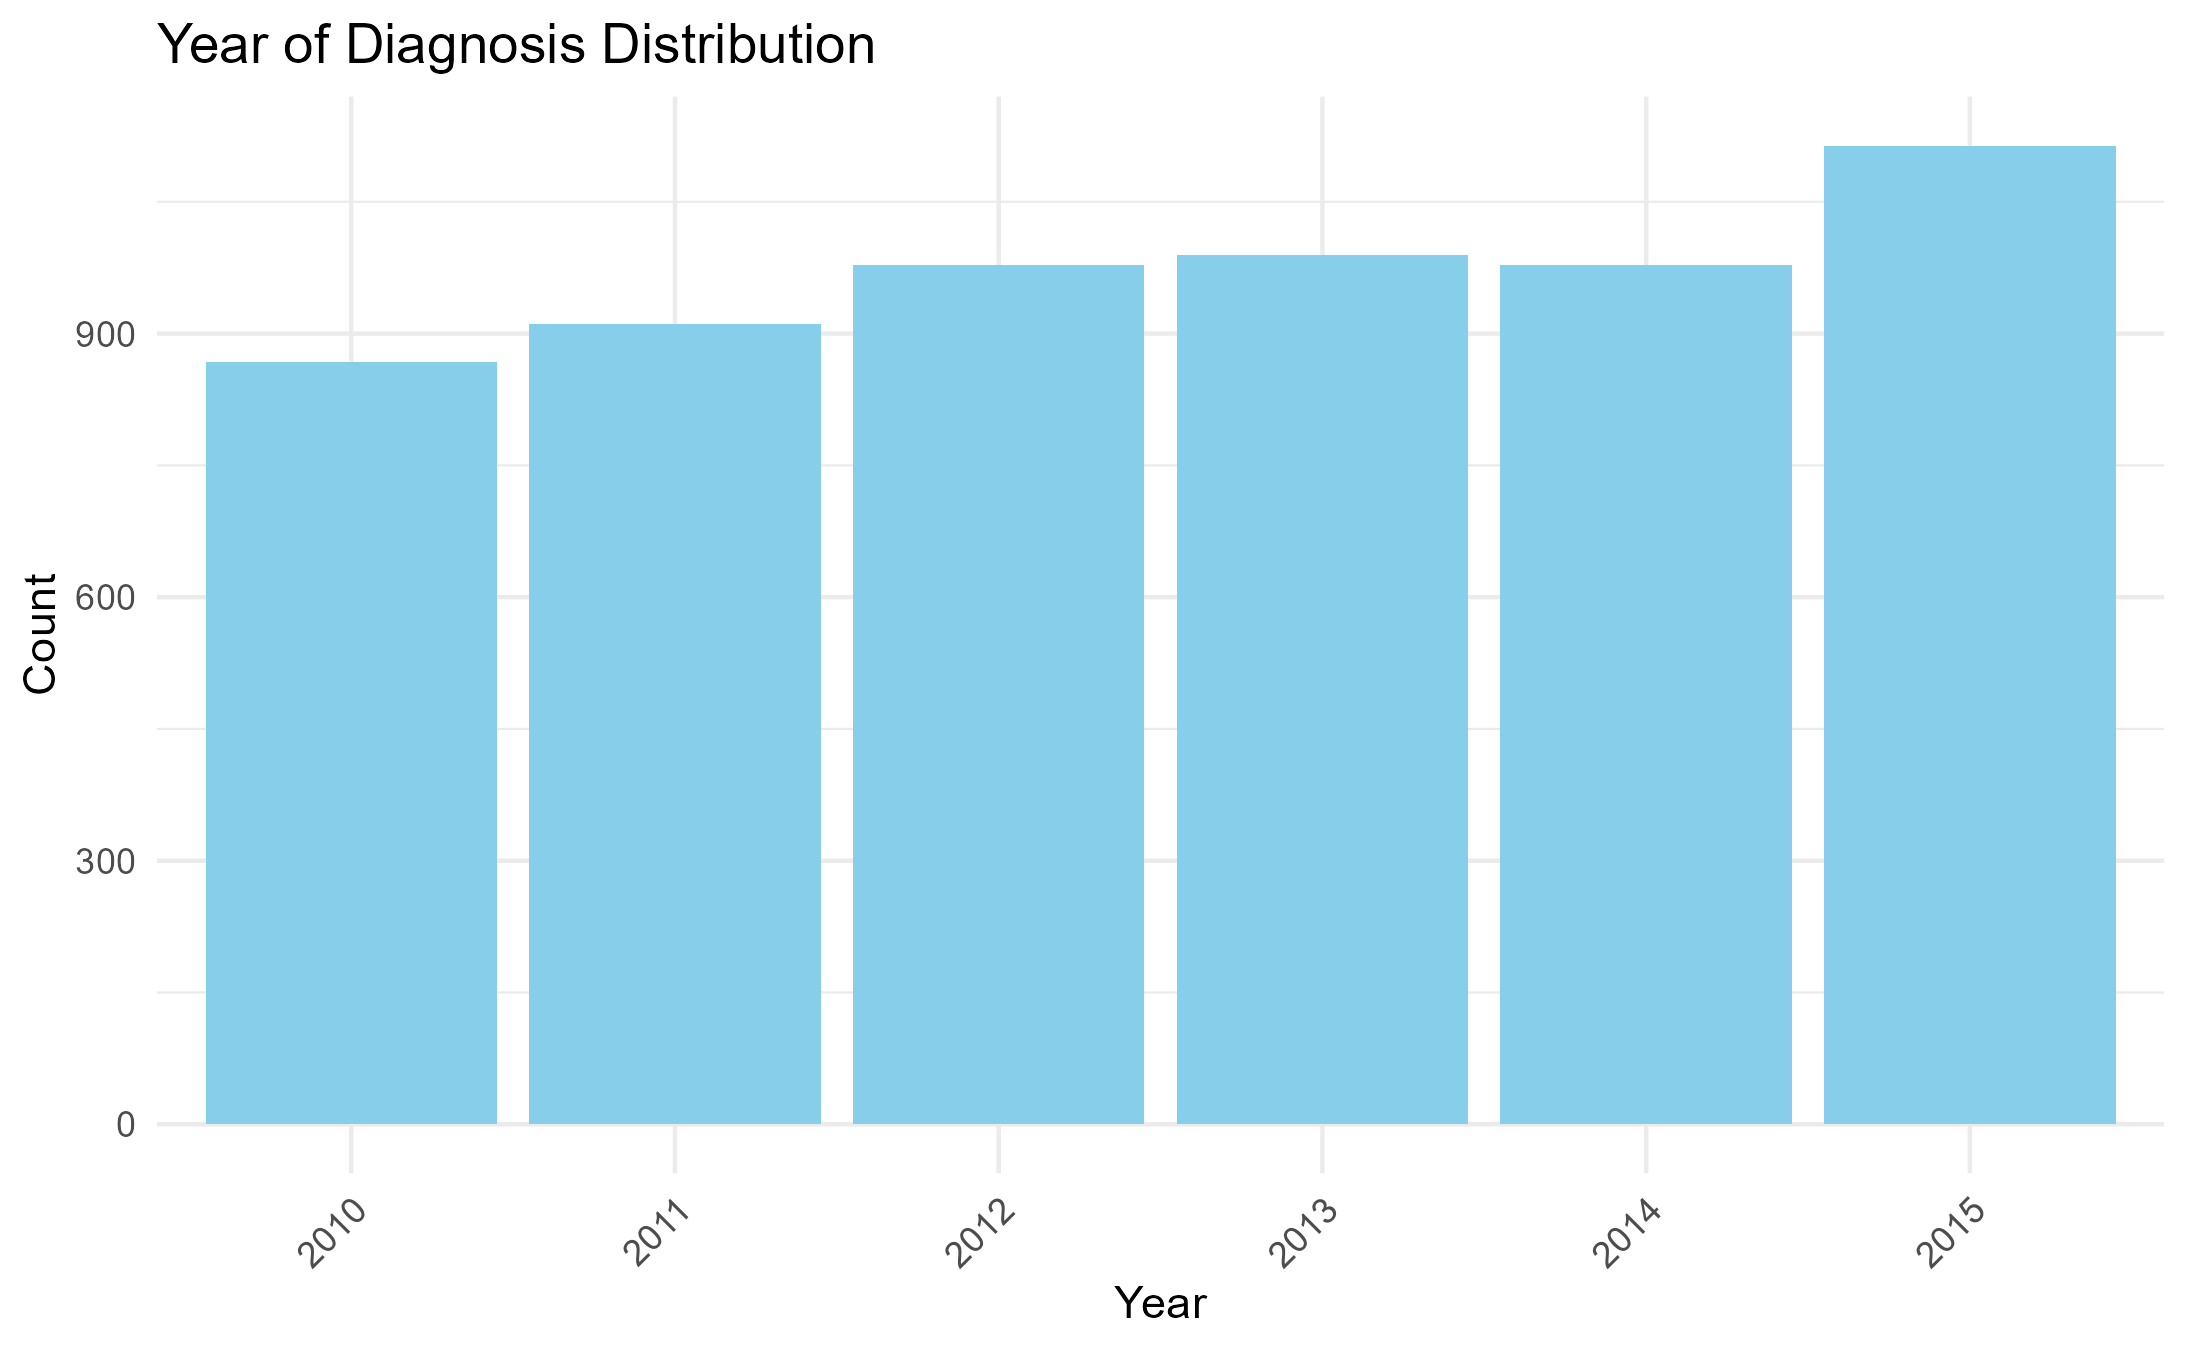
\includegraphics[width=7.29in,height=\textheight]{../../../results/edafigures/edayear.png}

}

\caption{\label{fig-year-diagnosis}Bar plot showing the distribution of
patients by year of diagnosis.}

\end{figure}%

\subsection{Exploratory Summary: Cause-Specific Death
Classification}\label{exploratory-summary-cause-specific-death-classification}

We summarized the distribution of outcomes according to the SEER
cause-specific death classification. The majority of patients in the
dataset (77.5\%) were classified as having died due to the primary
cancer diagnosis, while 22.5\% were either alive or had died from other
causes. This outcome classification was used as the primary event
definition in survival models throughout the analysis.

\begin{enumerate}
\def\labelenumi{\arabic{enumi}.}
\setcounter{enumi}{1}
\tightlist
\item
  Distribution of patients by cause-specific death classification.
\end{enumerate}

\begin{longtable}[]{@{}lrr@{}}

\caption{\label{tbl-cause-death}Cause-specific death classification
among patients in the cohort.}

\tabularnewline

\toprule\noalign{}
cause\_specific\_death & Count & Percentage \\
\midrule\noalign{}
\endhead
\bottomrule\noalign{}
\endlastfoot
Alive or dead of other cause & 1287 & 22.5 \\
Dead (attributable to this cancer dx) & 4421 & 77.5 \\

\end{longtable}

\subsection{Univariate Analysis}\label{univariate-analysis}

To evaluate whether survival outcomes varied over time, we conducted a
bivariate Cox proportional hazards analysis using year of diagnosis as
the predictor. The year 2010 was used as the reference category. Hazard
ratios (HRs) for each subsequent year (2011 to 2015) were calculated to
assess whether patients diagnosed in later years had different risks of
death compared to those diagnosed in 2010. As shown in
Table~\ref{tbl-year-diagnosis}, all HRs were close to 1, and none of the
comparisons reached statistical significance (all p \textgreater{}
0.05), indicating that there was no significant year-to-year variation
in survival over the study period. These findings suggest a relative
consistency in survival outcomes for patients diagnosed between 2010 and
2015 within this dataset.

\begin{longtable}[]{@{}lrrrr@{}}

\caption{\label{tbl-year-diagnosis}Hazard ratios from Cox regression
evaluating year of diagnosis and survival.}

\tabularnewline

\toprule\noalign{}
term & estimate & std.error & statistic & p.value \\
\midrule\noalign{}
\endhead
\bottomrule\noalign{}
\endlastfoot
diagnosis\_year2011 vs.~2010 & 0.981 & 0.054 & -0.368 & 0.713 \\
diagnosis\_year2012 vs.~2010 & 0.984 & 0.052 & -0.316 & 0.752 \\
diagnosis\_year2013 vs.~2010 & 1.000 & 0.053 & -0.001 & 1.000 \\
diagnosis\_year2014 vs.~2010 & 0.978 & 0.053 & -0.429 & 0.668 \\
diagnosis\_year2015 vs.~2010 & 0.982 & 0.052 & -0.349 & 0.727 \\

\end{longtable}

\subsection{Random Forest Model: Predicting Cause-Specific
Death}\label{random-forest-model-predicting-cause-specific-death}

We implemented a random forest classifier to predict whether a patient's
death was attributable to cancer using SEER registry variables. The
dataset was preprocessed with downsampling to address class imbalance.
We used 5-fold cross-validation to tune hyperparameters and selected the
best model based on ROC AUC. The model was trained on 80\% of the data
and evaluated on a held-out 20\% test set.

The top predictors, based on variable importance, included lung and
liver metastases, age group, and year of diagnosis.

Figure~\ref{fig-vip-rf} .Variable importance plot from the final tuned
random forest model. The top 10 predictors are displayed, with
mets\_lung and mets\_liver being the most influential variables for
predicting cause-specific death.

\begin{figure}

\centering{

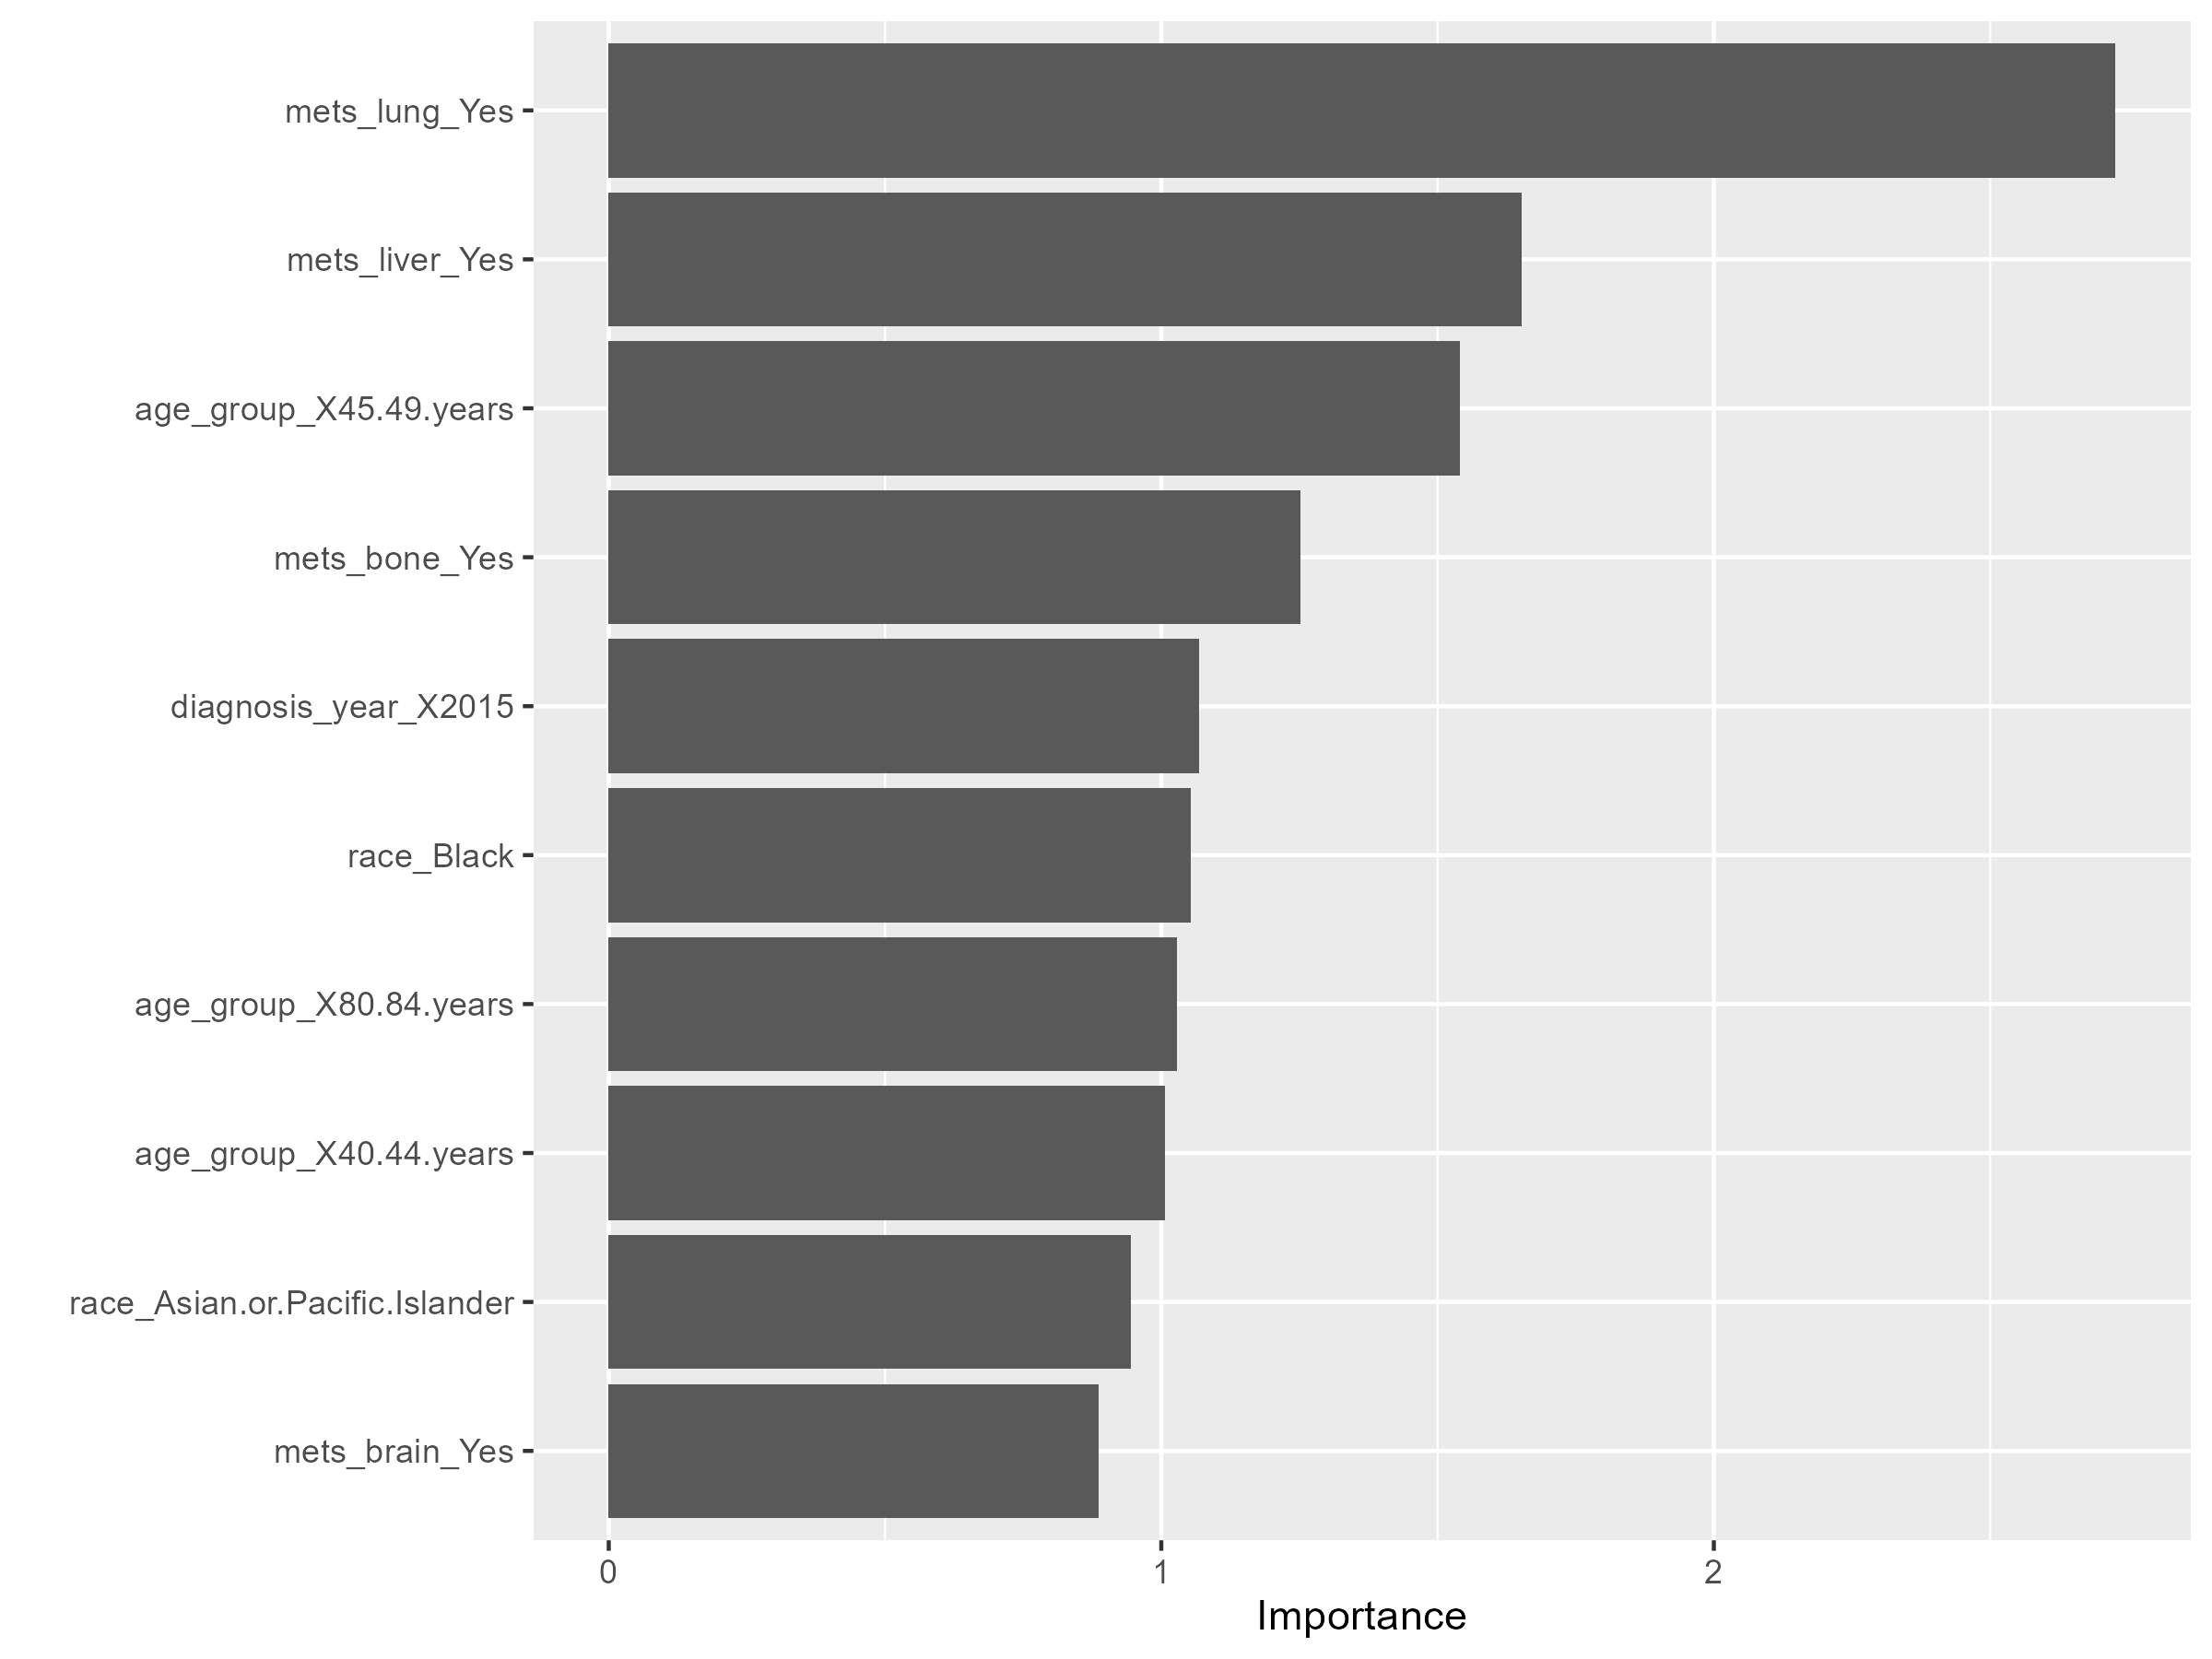
\includegraphics[width=8in,height=\textheight]{../../../results/figures/vip_plot_rf_balanced.png}

}

\caption{\label{fig-vip-rf}Top 10 most important variables from the
random forest model predicting cause-specific death.}

\end{figure}%

\begin{enumerate}
\def\labelenumi{\arabic{enumi}.}
\setcounter{enumi}{2}
\tightlist
\item
  Confusion matrix summarizing the random forest model's classification
  performance on the test set. The model shows better performance in
  identifying cancer-attributable deaths than non-cancer deaths,
  although overall accuracy was limited.
\end{enumerate}

\begin{table}

\caption{\label{tbl-rf-cm}Confusion matrix from the random forest model
on the test set.}

\centering{

\begin{verbatim}
$table
          Truth
Prediction  No Yes
       No  152 385
       Yes  92 447

attr(,"class")
[1] "conf_mat"
\end{verbatim}

}

\end{table}%

\begin{enumerate}
\def\labelenumi{\arabic{enumi}.}
\setcounter{enumi}{3}
\tightlist
\item
  Area under the receiver operating characteristic curve (ROC AUC) from
  the random forest model. The model achieved an AUC of approximately
  0.39, indicating limited discriminative performance, possibly due to
  overlapping features and class imbalance.
\end{enumerate}

\begin{table}

\caption{\label{tbl-rf-auc}ROC AUC score of the final random forest
model.}

\centering{

\begin{verbatim}
# A tibble: 1 x 3
  .metric .estimator .estimate
  <chr>   <chr>          <dbl>
1 roc_auc binary         0.394
\end{verbatim}

}

\end{table}%

\subsection{LASSO Cox Regression for Variable
Selection.}\label{lasso-cox-regression-for-variable-selection.}

To identify the most influential predictors of cancer-specific survival,
we applied LASSO (Least Absolute Shrinkage and Selection Operator)
penalized Cox regression using the glmnet package. This approach helps
in variable selection by shrinking less informative coefficients to zero
while retaining strong predictors. We performed 10-fold cross-validation
to select the optimal penalty parameter (λ), minimizing the partial
likelihood deviance.

\begin{enumerate}
\def\labelenumi{\arabic{enumi}.}
\setcounter{enumi}{4}
\tightlist
\item
  Selected variables from the LASSO model using the optimal penalty
  parameter (λ.min). These are the predictors that remained in the final
  model with non-zero coefficients.
\end{enumerate}

\begin{longtable}[]{@{}lr@{}}

\caption{\label{tbl-lasso-vars}Non-zero coefficients from the LASSO Cox
regression model.}

\tabularnewline

\toprule\noalign{}
variable & coefficient \\
\midrule\noalign{}
\endhead
\bottomrule\noalign{}
\endlastfoot
mets\_lungYes & 0.3323 \\
mets\_liverYes & 0.3862 \\
mets\_boneYes & 0.2833 \\
mets\_brainYes & 0.5570 \\
age\_group25-29 years & -0.1979 \\
age\_group30-34 years & -0.1054 \\
age\_group35-39 years & -0.2170 \\
age\_group40-44 years & -0.3530 \\
age\_group45-49 years & -0.1630 \\
age\_group50-54 years & -0.0678 \\
age\_group55-59 years & -0.0226 \\
age\_group60-64 years & 0.0159 \\
age\_group70-74 years & 0.2417 \\
age\_group75-79 years & 0.3073 \\
age\_group80-84 years & 0.4241 \\
age\_group85+ years & 0.6496 \\
raceBlack & 0.3345 \\
raceAsian or Pacific Islander & -0.0173 \\
raceAmerican Indian/Alaska Native & 0.1343 \\
median\_income\$40,000 - \$44,999 & 0.0456 \\
median\_income\$50,000 - \$54,999 & 0.0571 \\
median\_income\$65,000 - \$69,999 & 0.0468 \\
median\_income\$70,000 - \$74,999 & 0.0038 \\
diagnosis\_year2013 & 0.0283 \\
diagnosis\_year2014 & -0.0097 \\

\end{longtable}

\newpage{}




\end{document}
